\documentclass[12pt]{ruthesis}
%\documentclass[12pt]{amsart}
\usepackage{amsmath}
\usepackage{amssymb}
\usepackage{latexsym}
\usepackage{epsfig,epsf,rotating}
\usepackage{subfigure}
\usepackage{siunitx}
%\usepackage{pictex}
\usepackage{epsf}
\usepackage{theorem}
\usepackage{graphicx}
\usepackage{hyperref}
\usepackage{typedref}
\usepackage[version=3]{mhchem}
%\usepackage{cite}
\usepackage[numbers, sort&compress]{natbib}

\title{Microwave spectroscopy on two dimensional electron gas}
\ctitle{Microwave spectroscopy on two dimensional electron gas}
\author{Jie Zhang}
\department{Physics and Astronomy}
\school{Rice University}
\degree{Master of Science}

\committee {
		Rui-Rui Du\\
        Professor of Physics and Astronomy \and
        Junichiro Kono, Chair \\
        Professor of Electrical and Computer Engineering and Physics \& Astronomy \and
        Wei Li\\
        Associate Professor of Physics and Astronomy\and
       }

\address{Houston, Texas}
\donemonth{August} \doneyear{2015} \makeindex
\begin{document}

  \begin{frontmatter}
   \pagenumbering{roman}
   %\makecover
   \maketitle

\begin{abstract}

Microwave spectroscopy for detecting various resonance  of electrons is our main focus and we have been using electrical, thermal and absorption method for different purposes.  

Electron Spin Resonance (ESR) and Cyclotron resonance (CR) are two of the most significant feature of electrons under magnetic field where electrical detection requires contacts on the sample which usually causes damages. In order to detect the electron spin resonance (ESR) of a single nano-object, high sensitive tool is required. So far, the best commercial ESR detector can detect around 1000 spins. We develop an ultra-sensitive calorimeter which is aimed at resolving the ESR of one nano-object. As a pretest, we show that CR can be measured via heat generated by resonant absorption of photons. An increase in the lattice temperature can be detected when the energy of the incident microwave photons matches the energy difference between adjacent Landau levels. They will be absorbed converting to phonons via non-radiative relaxation. A nano-calorimetry is constructed which can operate at 300 mK and precision of our thermometer is improved to tens of micro-Kelvins, thereby increasing the sensitivity to several nano-watts. 

Edge state transport is also an interest of ours due to its pure one dimensionality and dissipationless feature. Microwave absorption spectroscopy of quantum droplet on two dimensional electron/hole gas is a powerful tool investigating the number and velocities of the charge modes. We have sample patterned with multiple circular dots on the order of several microns. It is directly placed onto the meander line superconducting waveguide positioned inside a resonance container. The whole setup is attached to the bottom of a top loaded Helium 3 cryostat with base temperature down to 300mK. This absence of quantum contact has the advantage over standard transport measurement with its high sensitivity and could be generalized to a common method probing edge states hosted in other new materials.

\begin{figure}
  \centering
  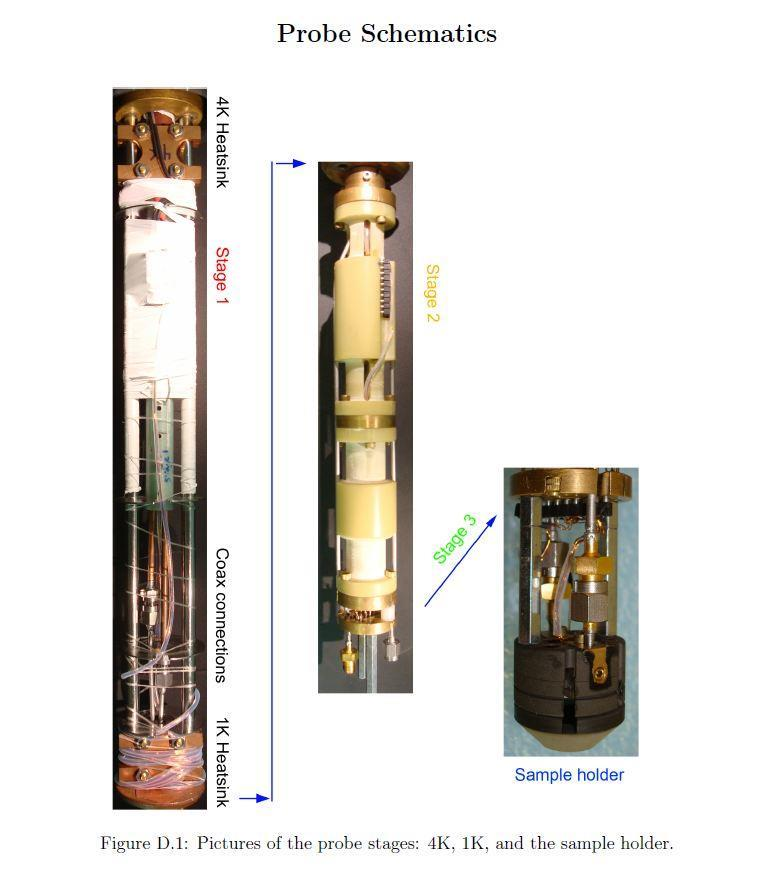
\includegraphics[totalheight=8cm]{figures/SomeImage.jpeg}
  \caption{This is a caption.}
  \label{fig:verticalcell}
\end{figure}

\end{abstract}

%\include{ack}
\tableofcontents
\listoffigures
%\listoftables
%   \include{ded}
\end{frontmatter}
\pagenumbering{arabic}
\linespacing{1.7}


\chapter{Introduction}\label{Intro}


\chapter{Transport behavior of electrons under the illumination of microwave}\label{Transport}

\section{SdH Oscillation and MIRO}\label{SdHO}
Shubnikov?de Haas oscillations

\section{Zero Resistance State}\label{ZRS}

\chapter{Thermal behavior of electrons under the illumination of microwave}\label{Thermal}

\section{Theoretical Support}\label{Theoretical}

\section{Setup Construction}\label{Construction}

\section{Cyclotron Resonance Pretest}\label{Cyclotron}

\section{Spin Resonance on DPPH}\label{DPPH}

\chapter{Microwave absorption spectroscopy of electrons in 2DEG}\label{Absorption}

\section{Setup Construction}\label{Construction}

\section{Cyclotron Resonance Pretest}\label{Cyclotron}

\section{Improvement underway}\label{Improvement}

\cite{Chen01APL}.
\figureref{Conductance}.



%\begin{figure}
%\includegraphics[scale=0.6]{Fig/Conductance.jpg}
%\caption{(a)~ Normalized conductance of an individual semiconducting SWCNT vs. time during UV illumination cycles in air.  (b)~Conductance response to UV illumination in $10^{-8}$ Torr vacuum~\cite{Chen01APL}.}
%\label{Conductance}
%\end{figure}



\chapter{Summary}\label{summary}





\appendix

%\include{append-a}
%\appendix
%\addcontentsline{toc} {chapter}{\numberline {}Appendix A}
%\include{append-a}
%\include{append-b}
%\addcontentsline{toc} {chapter}{\numberline {}Bibliography}{}
%\include{biblio}

\bibliographystyle{ieeetr}
\bibliography{Jie Zhang}
\end{document}
